\documentclass[12pt,twoside]{article}
\usepackage{jmlda}
\usepackage{hyperref}       % clickable links
\usepackage{Iv_commands}    % you can deletee this
\newcommand{\hdir}{.}
\renewcommand{\L}{\mathcal{L}}

% version 0.3.2

\title
    {Синергия алгоритмов классификации (SVM Multimodelling)}
\author
    {С.\,~Иванычев, А.\,~Адуенко}
\email
    {\href{mailto:sergeyivanychev@gmail.com}{sergeyivanychev@gmail.com},  \href{mailto:aduenko1@gmail.com}{aduenko1@gmail.com}}
\organization
    {Московский физико-технический институт}
\abstract
    {В данной статье рассматривается проблема агрегирования небольшого количества сильных классификаторов с целью улучшения решений задач классификации и регрессии.  В качестве примера подобной системы рассматривается система SVM  алгоритмов использующая kernel-trick с различными ядрами. Для комбинации решений и улучшения качества прогнозирования в задачах классификации и регрессии (SVR) авторы предлагают способ формирования новых признаков на основе сгенерированных отступов (\emph{margins}) каждым классификатором, приводят алгоритм обучения на полученных объектах и анализируют отличия множеств опорных объектов для различных ядер. В качестве практической проверки были проведены эксперименты на различных реальных данных из репозитория UCI.

    \bigskip
\noindent
\textbf{Ключевые слова}: \emph {двухклассовая классификация, композиция алгоритмов, SVM, SVR, бэггинг}
}

\bibliographystyle{unsrt}

\begin{document}
\maketitle

\section{Введение}
Работа посвящена комбинированию небольшого количества сильных SVM, использующих kernel-trick с различными ядрами и получению агрегированного классификатора для улучшения решений задач классификации и регрессии.

    SVM(Support Vector Machine) или \emph{метод опорных векторов}\cite{Cortes1995, Boser1992} ---~это один из наиболее распространенных и эффективных методов в машинном обучении, которые используется для задач классификации и регрессии (SVR). Задача математического программирования сводится к двойственной задаче, функционалы в которой не зависят от векторов признаков как таковых, а лишь от их попарных скалярных произведений \cite{Voron} . Использование особых функций, \emph{ядер}, то есть скалярных произведений в сопряженном пространстве, позволяет получить разделяющие поверхности между классами более сложной формы \cite{Smola2004}. Наша цель --- скомбинировать SVM
    с различными примененными ядрами для улучшения решения, а также анализ множеств опорных объектов в случае разных использованных ядер.

    Наиболее классическими методами агрегирования алгоритмов являются
    бэггинг (\emph{bagging})\cite{Breiman1996} и бустинг (\emph{boosting}) \cite{Freund1995}, и их
    вариации, однако они работают только с  большим количеством слабых классификаторов, что делает невозможным использование его использование для указанного множества базовых алгоритмов.

    Среди способов агрегации для небольшого количества классификаторов можно
    выделить, например, выбор большинства классификаторов \cite{Franke1992},
    комбинирование ранжирований (rankings) по классам, сделанных различными
    классификаторами \cite{Ho1994}. В дальнейшем было показано, что все подобные
    методы есть особые случаи составного классификатора из \cite{Kittler1996},
    появляющиеся при особых условиях или способах аппроксимации.

    Различные способы агрегации SVМ используются во многих задачах анализа данных.
    \cite{Martin-merino2007} использовали совокупность SVМ для уменьшения ошибочно негативных классификаций (FP) в задаче фильтрации спама среди электронных писем.
    Для этого на электронных письмах были введены различные метрики, для каждой из них был приспособлен SVM, а затем результат получался голосованием \cite{Kittler1996}.
    \cite{Gorgevik2005}, решавшие задачу распознавания написанных рукой символов, делили множество признаков на четыре непересекающихся подмножества, и на каждом из них обучали SVM, увеличив этим самым коэффициент распознавания по сравнению с одним SVM.

    В последнее время стал набирать популярность \emph{метод многоядерного обучения} (MKL,~multiple kernel learning) \cite{Dyrba2015, Bucak2014,Althloothi2014}, который основывается на том, что линейная комбинация ядер также является ядром. Данный метод хорош при объединении данных из нескольких источников и полной автоматизации, так как суперпозиция функций может быть оптимизирована любым методом валидации (например кросс-валидацией).

    Мы также предлагаем использовать накопившийся банк ядер, однако не на этапе обучения SVM, а на этапе агрегирования обученных алгоритмов. Известно, что алгоритм $b_i$ для объекта $x_j$ обучающей выборки генерирует \emph{отступ} (margin). По отступу в общем случае можно определить не только предсказанный класс, но и насколько <<уверен>> в своем решении алгоритм. В случае банка с $n$ ядрами и обучающей выборки с $m$ сэмплами
    мы получим матрицу отступов $M \in \R^{m\times n}$. Отнормировав ее, мы получим новую матрицу <<объект-признак>>, где вектором признаков каждого объекта будет вектор отнормированных отступов.

    В этой работе предложен алгоритм обучения на матрице отступов, проведен анализ опорных объектов, генерируемые различными ядрами, а также проведено тестирование полученного алгоритма на реальных данных репозитория UCI.


\section{Постановка задачи}

Пусть $X^l = \brs{\vec{x}_i, y_i}_{i=1}^l$~---~обучающая выборка, $\vec{x}\in \R^n, y \in Y$ где $|Y| < \infty$~--- задача классификации, $|Y| = \infty$ --- задача регрессии. В данной статье под $s$-й \emph{моделью} будем понимать SVM с
ядром $K_s$ где выбрано множество ядер:

$$
\mathcal{K} = \{K_i\}_{j=1}^m
$$

При обучении каждая модель дает классификатор или регрессор (в зависимости от типа $Y$). Например, для случая $Y \in \{-1, +1\}$ классификации алгоритм выглядит следующим образом:

$$
b_s(\v{x}) = \sign{\sum_{i=1}^l\lambda_i y_i K_s(\vec{x}_i, \vec{x}) - w_0}
$$

Где $\{\lambda_i\}$ и $w_0$ находятся из решения задачи математического программирования\cite{Smola2004}

\begin{equation*}
 \begin{cases}
   \sum_{i=1}^l \lambda_i + \frac{1}{2}\sum_{i=1}^{l}\sum_{j=1}^{l}
    \lambda_i \lambda_j y_i y_j K_s(\vec{x}_i, \vec{x}_j) \to \min_\lambda
   \\
   0 \leq \lambda_s \leq c, \;\; i = 1\ldots l
   \\
   \sum_{i=1}^l\lambda_i y_i = 0
 \end{cases}
\end{equation*}

Побочным результатом обучения является то, что модель для обучающей выборки генерирует вектор \emph{отступов} (margins) для каждого объекта.

Если мы рассмотрим множество моделей, обученных на $X^l$, то мы получим матрицу отступов  размерности
$M \in \R^{l\times m}$,
в котором $(i, j)$-й элемент ---~это отступ $i$-го объекта в SVM с~$j$-м ядром.

Пусть $M$ --- матрица <<объект-признак>>, $\mathcal{A}$ ---~ множество алгоритмов
вида
\begin{equation}
    \mathcal{A} = \fbrs{a(\vec{x}) = g(\vec{x}, \theta)|\theta \in \Theta}\;\; g:\R^m \to Y
\end{equation}

Пару $(g, \mathcal{K})$ назовем \emph{мультимоделью}.
$\L(y, y^*)$ ---~функционал качества, тогда перед нами стоит задача минимизации

\begin{equation}
    L(y, g(M, \theta)) \to \min_{\mathcal{A}, \Theta}
\end{equation}

%
% \section{Старая постановка задачи}
%
%
%
% Пусть $\mathcal{K} = \{K_i\}_{j=1}^m$ ---~множество ядер, выбранных для
% мультимоделирования SVM, $X^l = \brs{\vec{x}_i, y_i}_{i=1}^l$~---~обучающая выборка$, \vec{x}\in \R^n, y \in Y$. Тогда множество обученных SVM на данной выборке:
%
% \begin{equation}
%     \mathcal{B} = \fbrs{b_i| b_i = b_i(\vec{x}) = \sign{\sum_{i=1}^l\lambda_i y_i K_i(\vec{x}_i, \vec{x}) - w_0}}_{i=1}^m
% \end{equation}
%
% Где $\lambda_s$ находятся из решения задачи математического программирования
%
% \begin{equation*}
%  \begin{cases}
%    \sum_{i=1}^l \lambda_i + \frac{1}{2}\sum_{i=1}^{l}\sum_{j=1}^{l}
%     \lambda_i \lambda_j y_i y_j K_s(\vec{x}_i, \vec{x}_j) \to \min_\lambda
%    \\
%    0 \leq \lambda_s \leq c, \;\; i = 1\ldots l
%    \\
%    \sum_{i=1}^l\lambda_i y_i = 0
%  \end{cases}
% \end{equation*}
%
% И $w_0 = \sum_{i=1}^l \lambda_i y_i K_s(\vec{x}_i, \vec{x}_j) - y_j$ для такого $j$, что
% $\lambda_j > 0, M_j = 1$. Паре <<выборка-обученные алгоритмы>> соответствует матрица отступов размерности
% $M \in \R^{l\times m}$,
% в котором $(i, j)$-й элемент ---~это отступ $i$-го объекта в SVM с~$j$-м ядром.
% Пусть $M$ --- матрица <<объект-признак>>, $\mathcal{A}$ ---~ множество алгоритмов
% вида
% \begin{equation}
%     \mathcal{A} = \fbrs{a(\vec{x}) = g(\vec{x}, \theta)|\theta \in \Theta}\;\; g:\R^m \to Y
% \end{equation}
%
% $\L(y, y^*)$ ---~функционал качества, тогда перед нами стоит задача минимизации
%
% \begin{equation}
%     L(y, g(M, \theta)) \to \min_{\mathcal{A}, \Theta}
% \end{equation}


\section{Базовый вычисительный эксперимент}

В данной секции попробуем установить связь между корреляцией векторов отступов,
генерируемых
разными ядрами на одной и той же обучающей выборке и степенью <<похожести>>
ядер. Понятие <<похожести>> или близости отождествляется с введением метрики
на пространстве ядер. Эту метрику терминах конкретной обучающей выборки можно
задать, например, нормализованной симметрической разностью множеств опорных объектов

$$
\rho_{X^l}(K_i, K_j) = \frac{\#\sbrs{\mathrm{SV}_i \;\Delta\; \mathrm{SV}_j}}
{\#\sbrs{\mathrm{SV}_i \cup \mathrm{SV}_j}}
$$

Где под $\mathrm{SV}_j$ понимается множество опорных объектов на $j$-м ядре, под
знаком $\Delta$ --- симметрическая разность. В качестве исходных данных
возьмем датасеты Wine \cite{UCI:Wine}, German credit data\cite{UCI:German} и
Heart disease\cite{UCI:Heart}. Варьируя коэффициент регуляризации,
 качестве базового набора ядер возьмем

\begin{itemize}
    \item Линейное
    \item Полиномиальное (степени 3, 4, 5)
    \item RBF-ядро ($\gamma \in \{0.0001, 0.001, 0.01, 0.1, 1\}$)
\end{itemize}

Для каждого значения коэффициента регуляризации построим графики

\newpage

\begin{figure}[H]
      \center{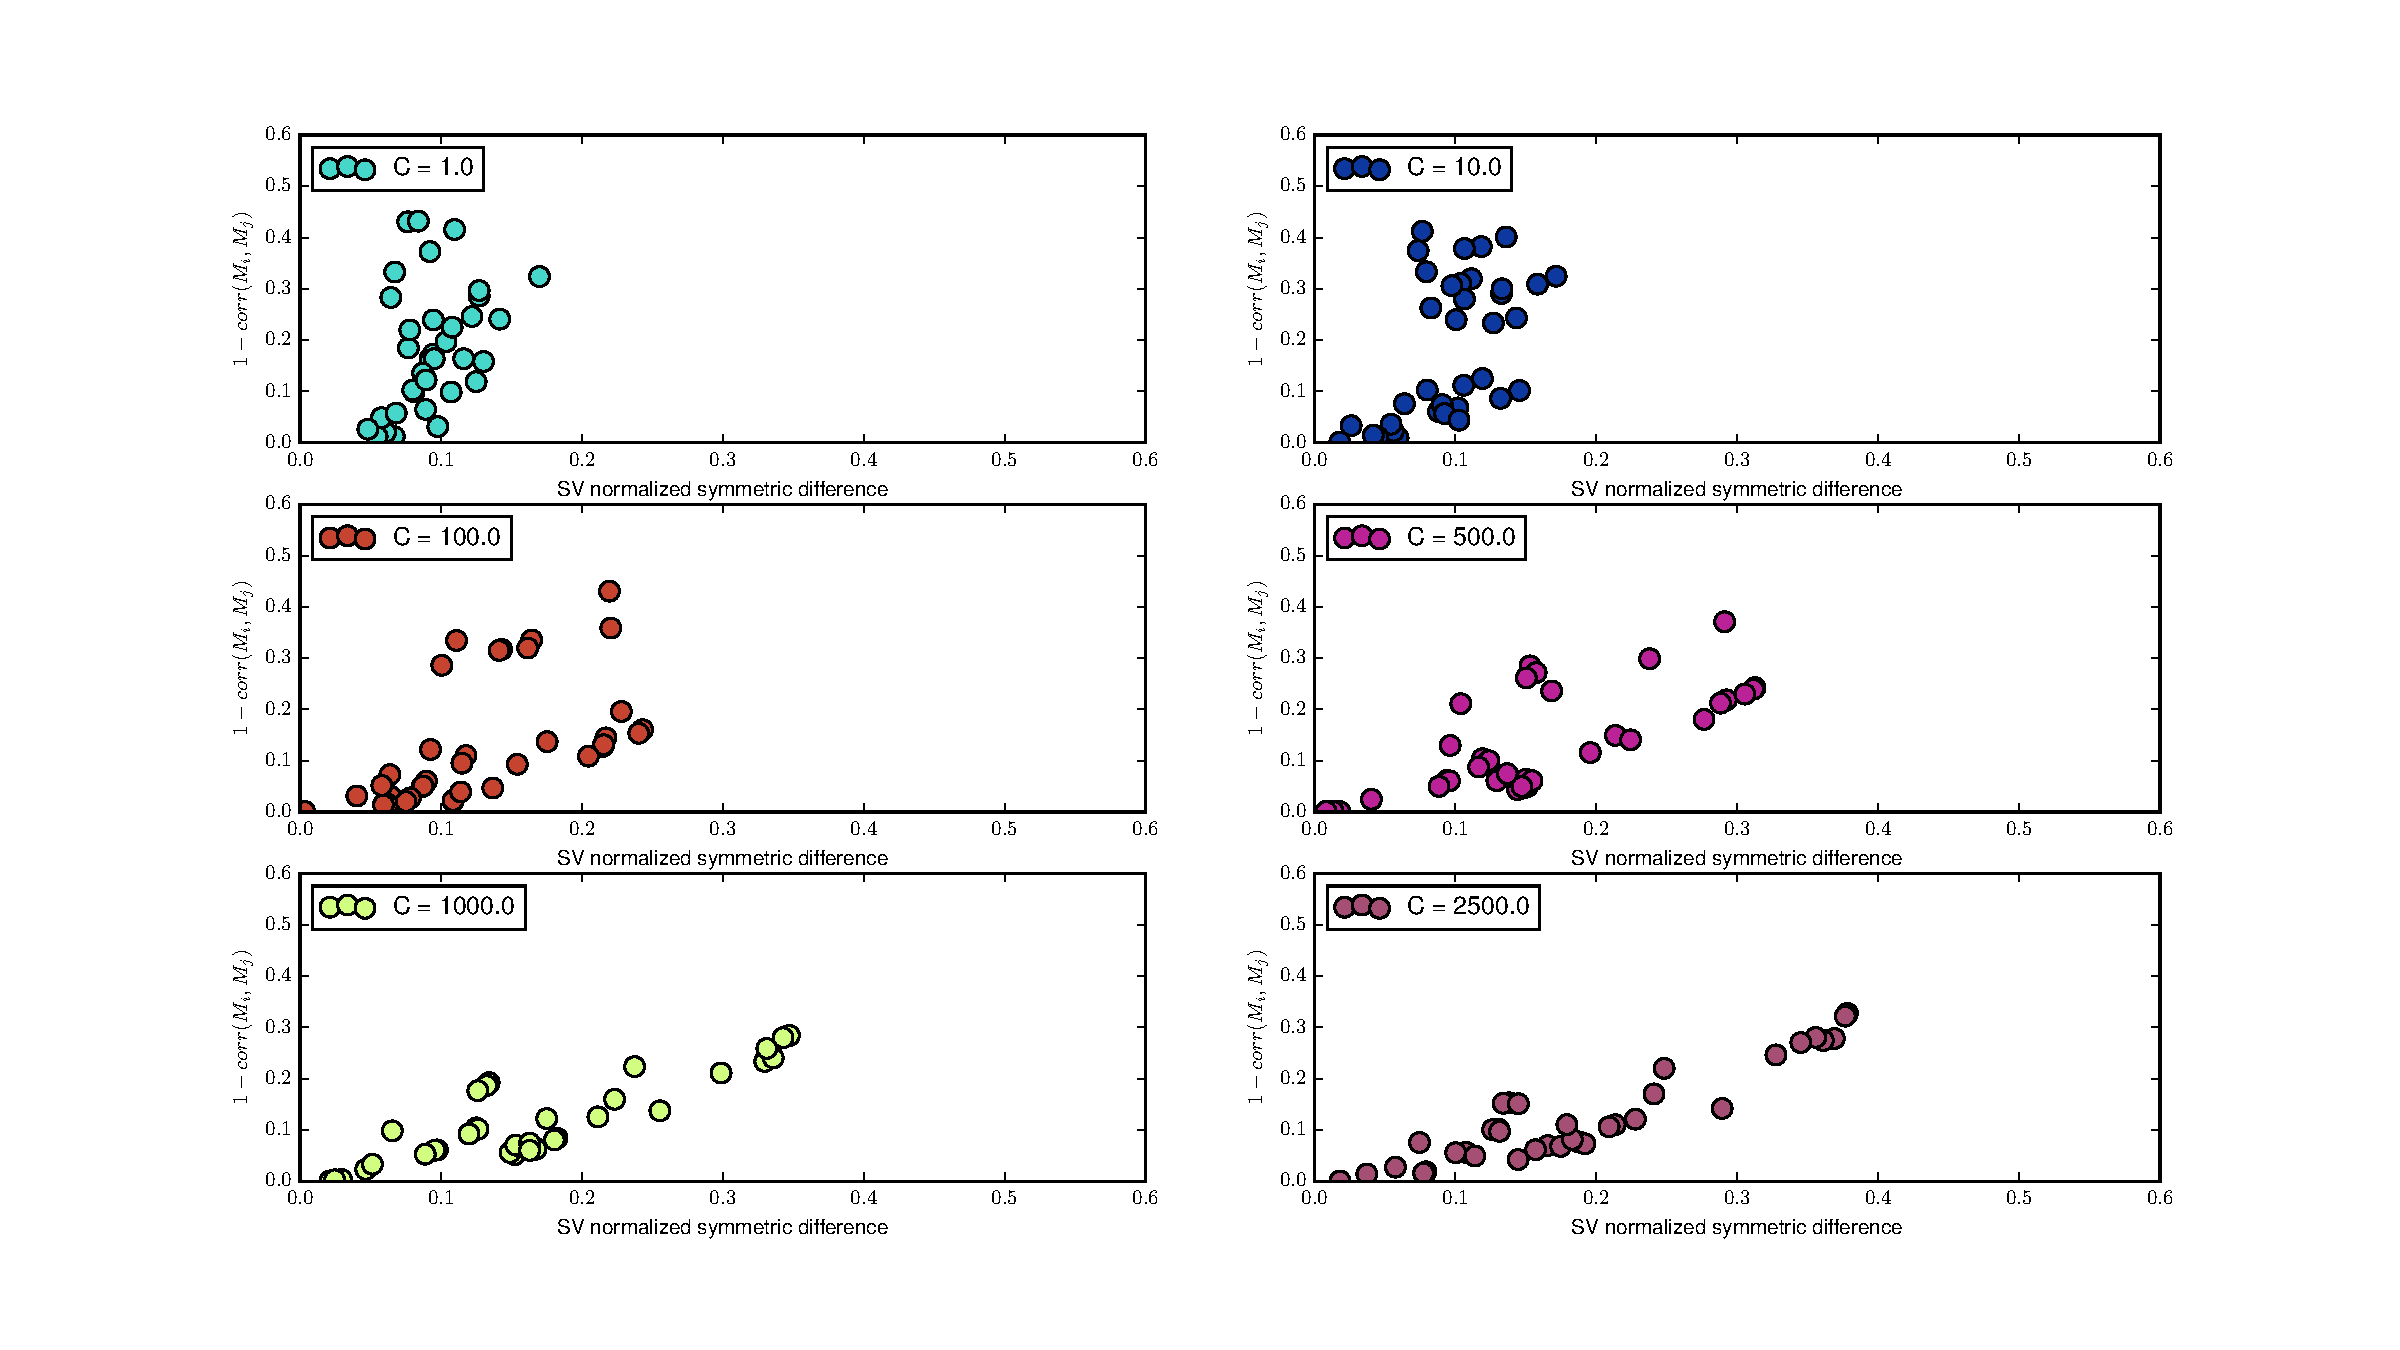
\includegraphics[width=\textwidth]{german.pdf}}
      \caption{German credit}
\end{figure}

\begin{figure}[H]
      \center{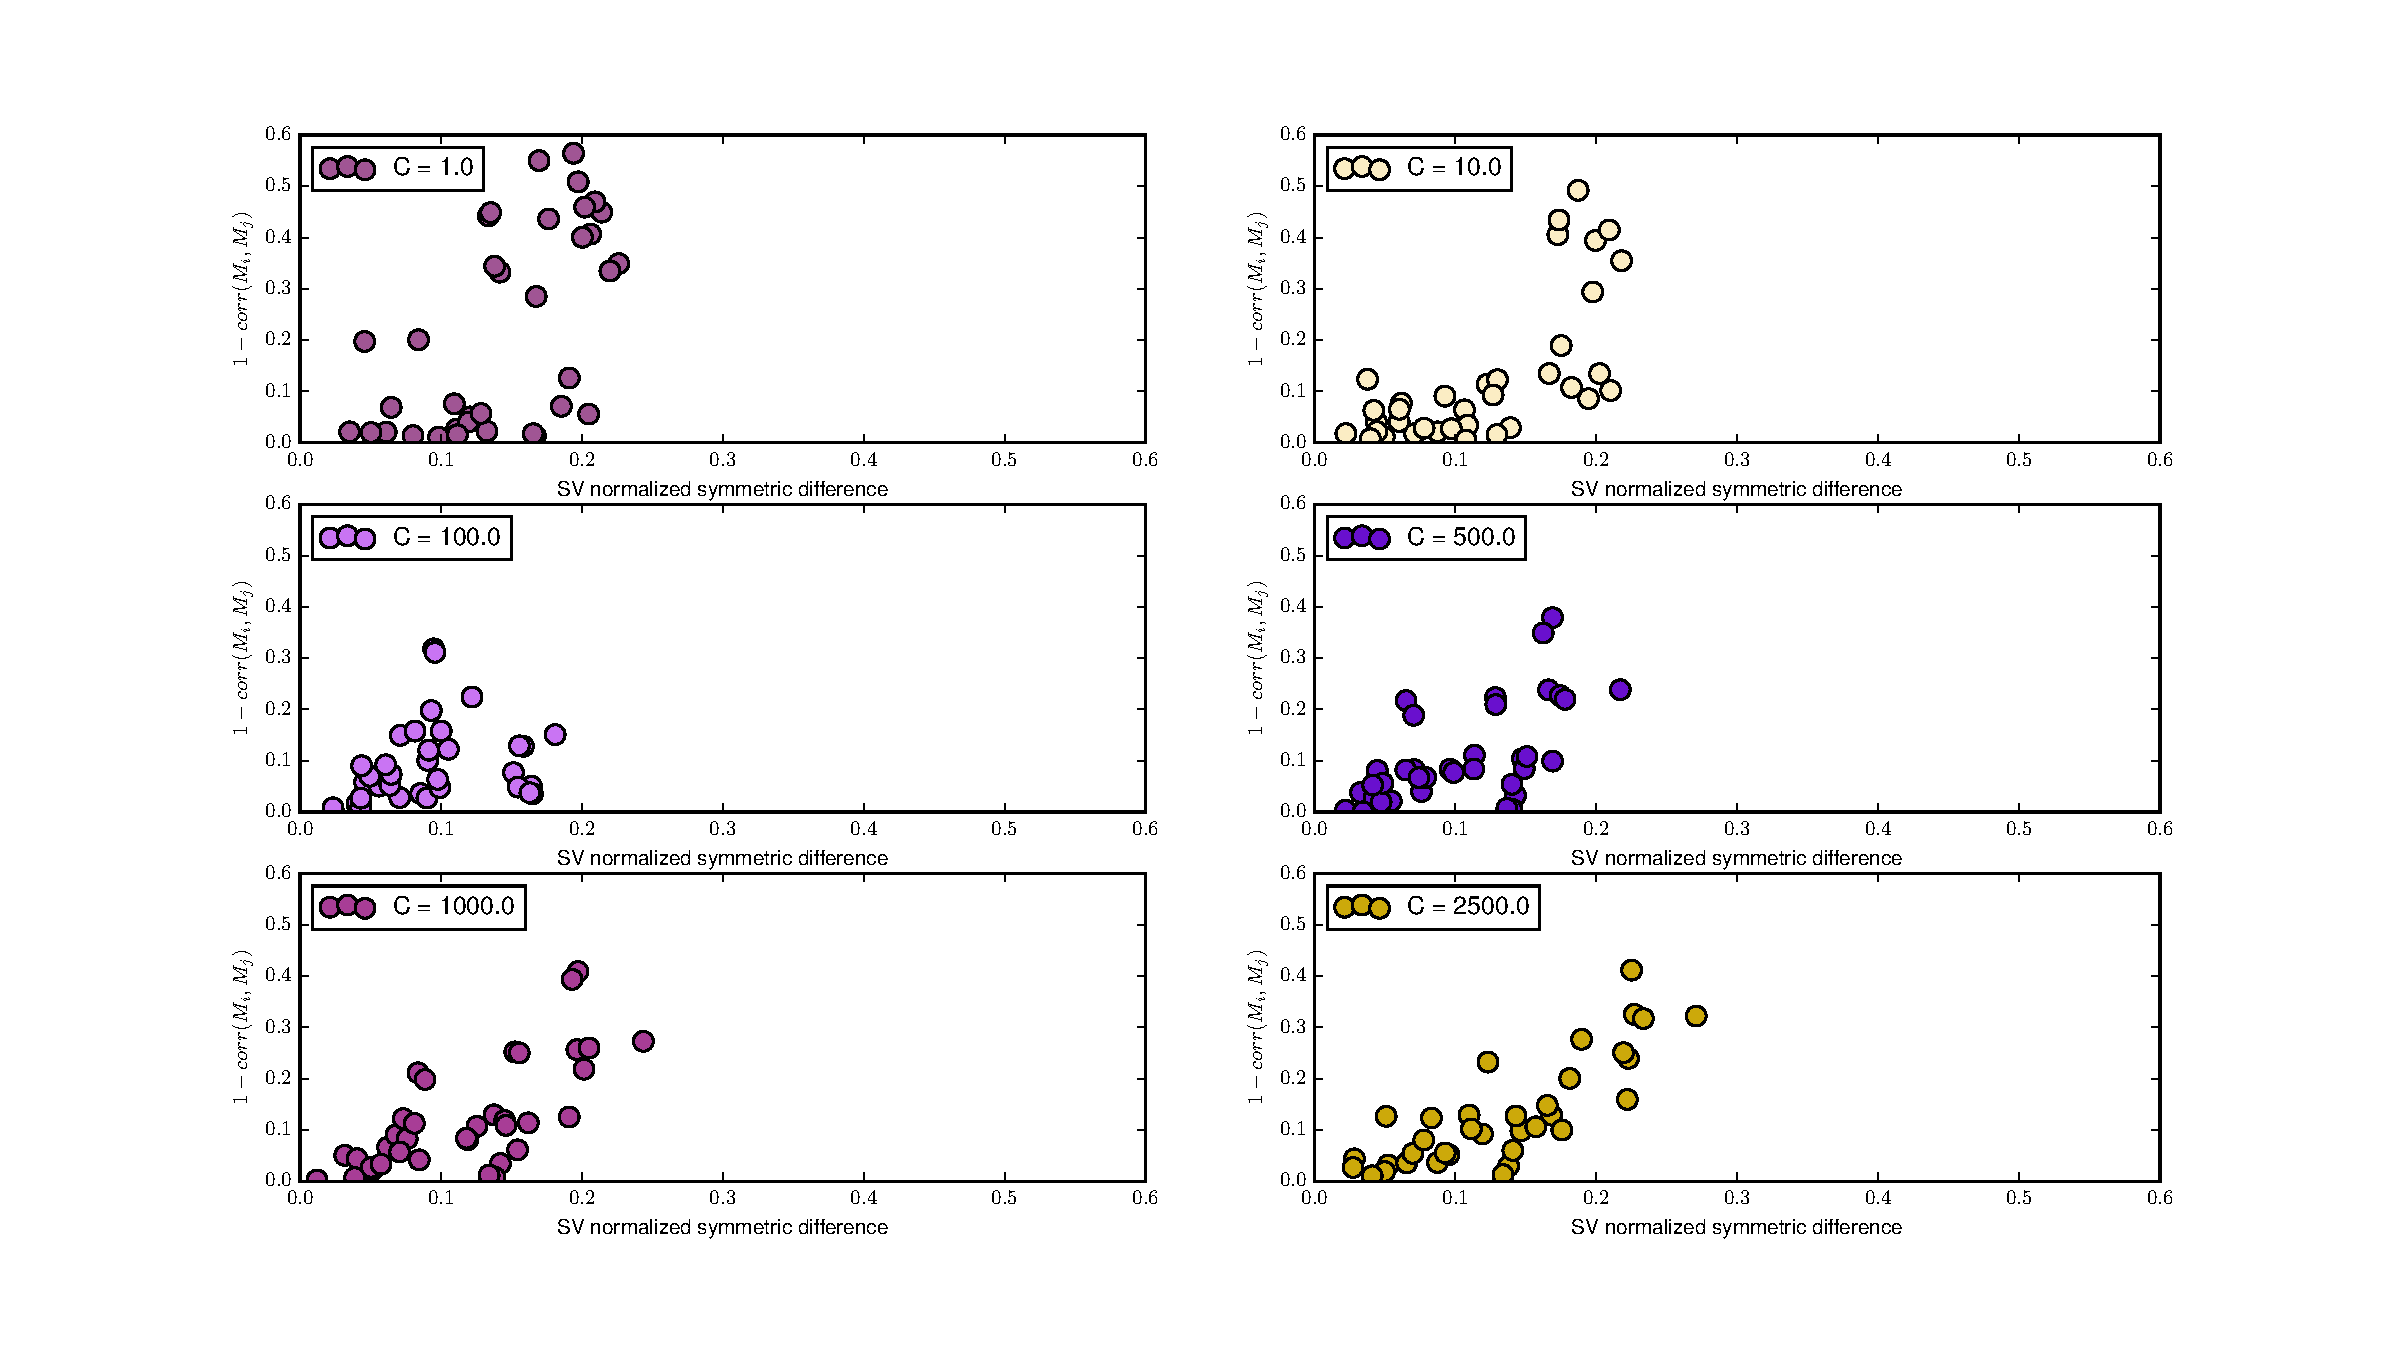
\includegraphics[width=\textwidth]{wine.pdf}}
      \caption{Wine quality}
\end{figure}

\begin{figure}[H]
      \center{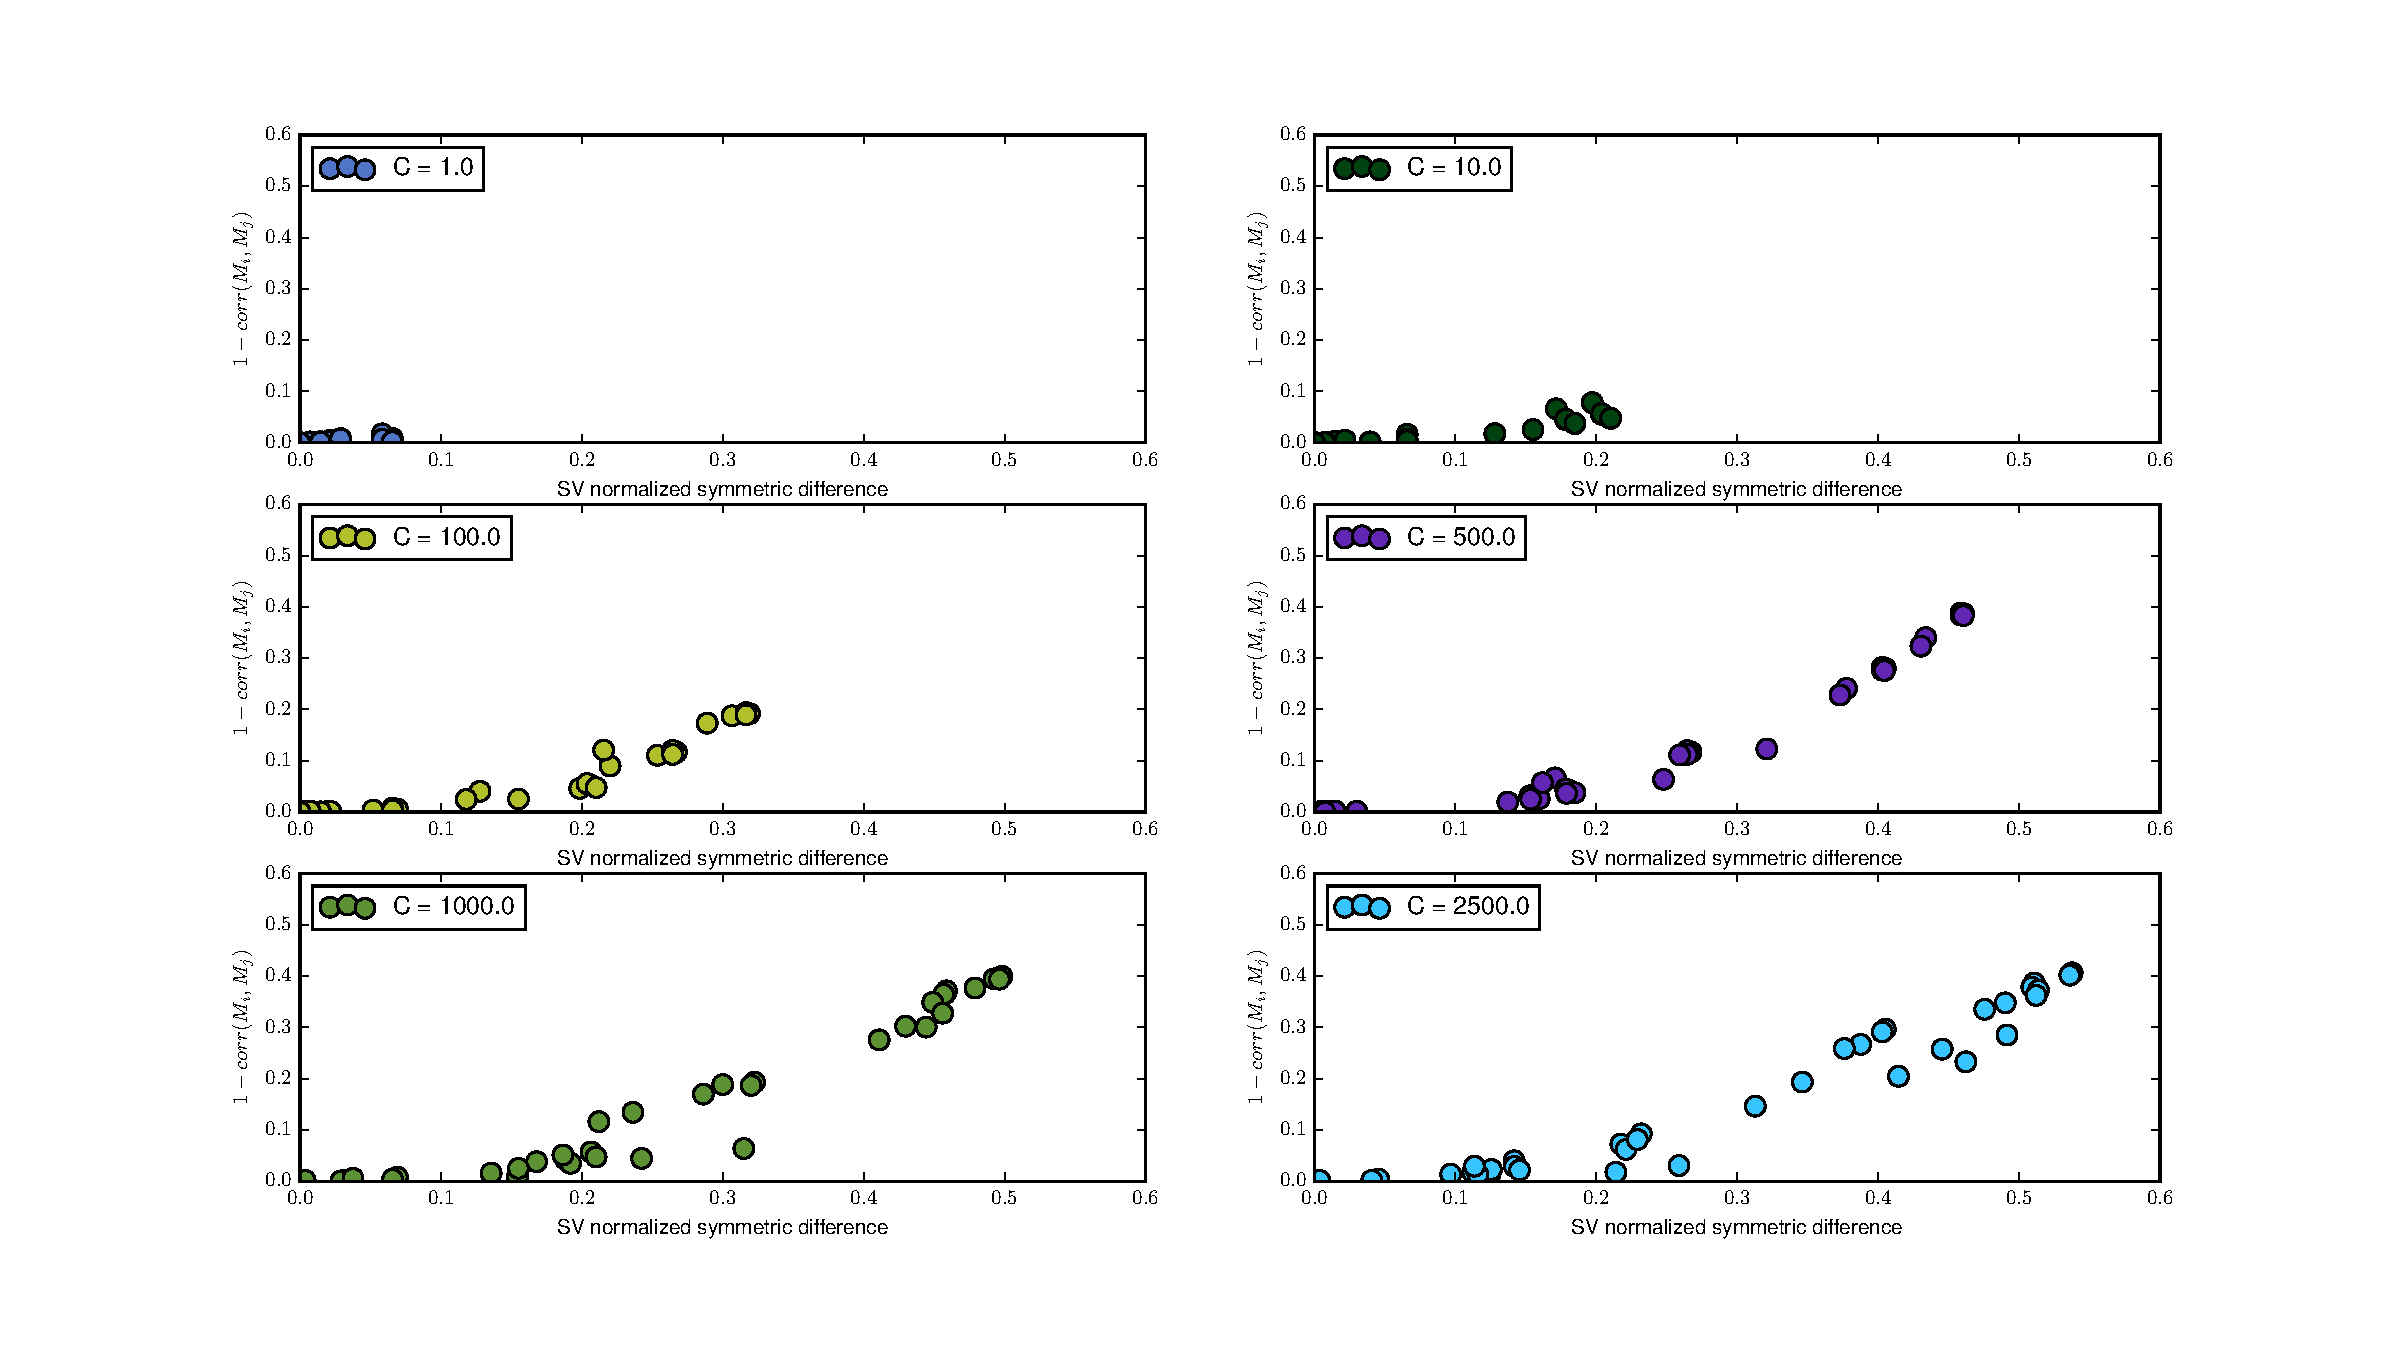
\includegraphics[width=\textwidth]{heart.pdf}}
      \caption{Heart disease}
\end{figure}

\bibliography{papers}

\end{document}
